\documentclass[a4paper,11pt]{article}

\usepackage[french]{babel}
\usepackage[T1]{fontenc}
\usepackage[utf8]{inputenc}
\usepackage{graphicx}
\usepackage{hyperref}
\usepackage{amsmath}
\usepackage{amssymb}
%\usepackage{fullpage}

\begin{document}

\title{\textbf{Compte rendu du TP \no 2}\\Méhode d'enrichissement de codes graphiques}
\author{Thibaut Castanié\\\textit{M2 IMAGINA}}
\date{\today}

\maketitle
\thispagestyle{empty}

\newpage 

\section*{Encodage d'un message en utilisant un CCE}

Multiplication d'une matrice avec un vecteur (exemple) :

\[\begin{bmatrix}1 & -1 & 2\\0&-3&1\end{bmatrix}\begin{bmatrix}2\\1\\0 \end{bmatrix} = \begin{bmatrix}1 \\-3 \end{bmatrix}\]

Fonction d'encodage de message en utilisant Hamming [7,4,3] :

\begin{itemize}
\item Entrée : \texttt{1011}
\item Sortie : \texttt{0110011}
\end{itemize}
On utilise la multiplication entre la matrice et le vecteur réalisée pour encoder le message, en multipliant la matrice de base et le message (en tant que vecteur).

\newpage

\section*{Personnalisation d'un code graphique}

\begin{center}
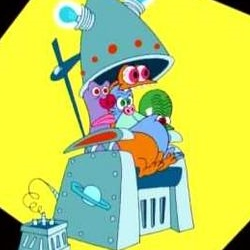
\includegraphics[scale=1]{zinzins.jpg}\\
\textit{Image personnalisée choisie}
\end{center}

\begin{center}
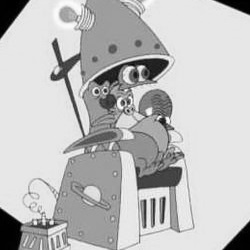
\includegraphics[scale=1]{zinzinsNB.jpg}\\
\textit{Image en niveaux de gris}
\end{center}

\begin{center}

\includegraphics[scale=1]{qrcode.jpg}\\
\textit{QR Code choisi}
\end{center}

\begin{center}
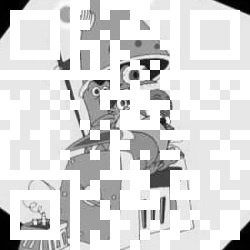
\includegraphics[scale=1]{fusion.jpg}\\
\textit{Assemblage de l'image et du QR Code}
\end{center}





\end{document}